\documentclass[letterpaper, 11pt]{article}
\usepackage[margin=1in]{geometry}
\usepackage{url, float, amsmath, amssymb}
\usepackage{fancyhdr}
\usepackage{graphicx}
\usepackage{titlesec}
\usepackage{hyperref}
\usepackage{caption}
\usepackage{hyperref}
\usepackage{setspace}
\usepackage[skip=2pt]{subcaption}
\usepackage[export]{adjustbox}

% bibliography packages
\usepackage[square,numbers]{natbib}
\bibliographystyle{plainnat}

\setcounter{secnumdepth}{4}

\titleformat{\paragraph}
{\normalfont\normalsize\bfseries}{\theparagraph}{1em}{}
\titlespacing*{\paragraph}
{0pt}{3.25ex plus 1ex minus .2ex}{1.5ex plus .2ex}

\title{\Large{\textbf{Statistics Applied Qualifying Review}}}

\author{Charlotte Mann}

\begin{document}

\setcounter{page}{1}

\pagestyle{fancy}
\fancyhead{}
\fancyhead[R]{\slshape \leftmark}

\maketitle
\onehalfspacing

\section{Introduction}

Mortality rates are certainly on the mind at the moment, with mortality counts reported daily due to the Covid-19 pandemic. Even outside of these unique times, mortality rates in the United States as a whole and for different demographic groups are of interest to understand the health of residents in the U.S. Understanding patterns in mortality can also help identify certain groups who should be targeted for interventions.

In this report, we are first interested in describing patterns in monthly mortality rates among the U.S. population between 2007 and 2018 by sex, age, year, and month. To do this, we fit linear regression models of the number of deaths per 100,000 people on different sets of covariates with interaction terms in order to tease out whether trends in mortality rates are consistent over time and if these trends differ according to other demographic factors.

After better understanding how the variability in mortality rate in the U.S. may be explained by time and demographic factors, we next are interested in how accurately we can predict mortality based on limited demographic factors and how the prediction accuracy may vary for different demographic groups. Predicting mortality is of interest since mortality counts take time to gather. Additionally, we expect that the current mortality predictions during the Covid-19 pandemic must take into account predictions of mortality were there not a pandemic, which provides motivation for this exercise. We compare the performance of four different models to predict mortality rate.


\section{Data}

We use data of monthly mortality counts (\texttt{deaths}) by year, age group, and sex for the years 2007 - 2018. The data is compiled from data gathered by the Center for Disease Control and Prevention's National Center for Health Statistics \cite{cdc_mort}. There is no missing data, so there are 12 months x 12 years x 18 age groups x 2 sexes = 5,184 observations. The data also included the total U.S. population value (\texttt{population}) for a certain age group, sex, and year (note this is not at the monthly level), from the US Census Bureau. The age variable is a factor variable with ages given in five year increments from age 0 - 84 years, and the last group including ages 85-99 years.

No data cleaning was necessary, although we do calculate our main response variable: number of deaths per 100,000 people in the population (we will refer to this value interchangeably as ``mortality" or ``mortality rate" as well through the rest of the report). We use the number of deaths per 100,000 people since it has nicer interpretability in our models than a raw proportion mortality rate and this measure is used by the CDC in their reports on mortality rates \cite{cdc_2018}. The number of deaths per 100,000 people is calculated as \texttt{deaths/population*100,000}. We assume that both the death counts and population counts represent the same population of residents of the United States, and thus that the population counts are appropriate to use as the denominator in our calculation of monthly mortality rates.\footnote{We note that the population values are for an entire year, rather than at the monthly level, but population values may vary from month to month for a variety of factors (births, deaths, immigration, emigration, etc.), that we do not have access to under the time constraint, so we do not try to infer monthly population values.}

Thus, our models only rely on these six variables: mortality per 100,000 population, year, month, age group, sex, and population count. We chose to include month as a factor variable separately from year in our models, since we want to isolate the effect of month separately from year. We additionally maintain age group as a factor variable (rather than coding it numerically) in our models since initial EDA indicates that there is not a linear relationship between age and mortality and the coefficients for individual age groups are easily interpretable.

\section{Exploratory data analysis of trends in mortality}\label{eda}

The number of deaths per 100,000 population range from .5 to 1719 people, with a mean of 155 people and a 75\% quantile of 135 people. In order to fit appropriate models, we first explore visual trends in mortality in the raw data. Since there are so few covariates, we are in the unique position of being able to plot all covariates at once and get a reasonable sense for trends and therefore which interactions to explore in our models.

\begin{figure}[h]
    \centering
    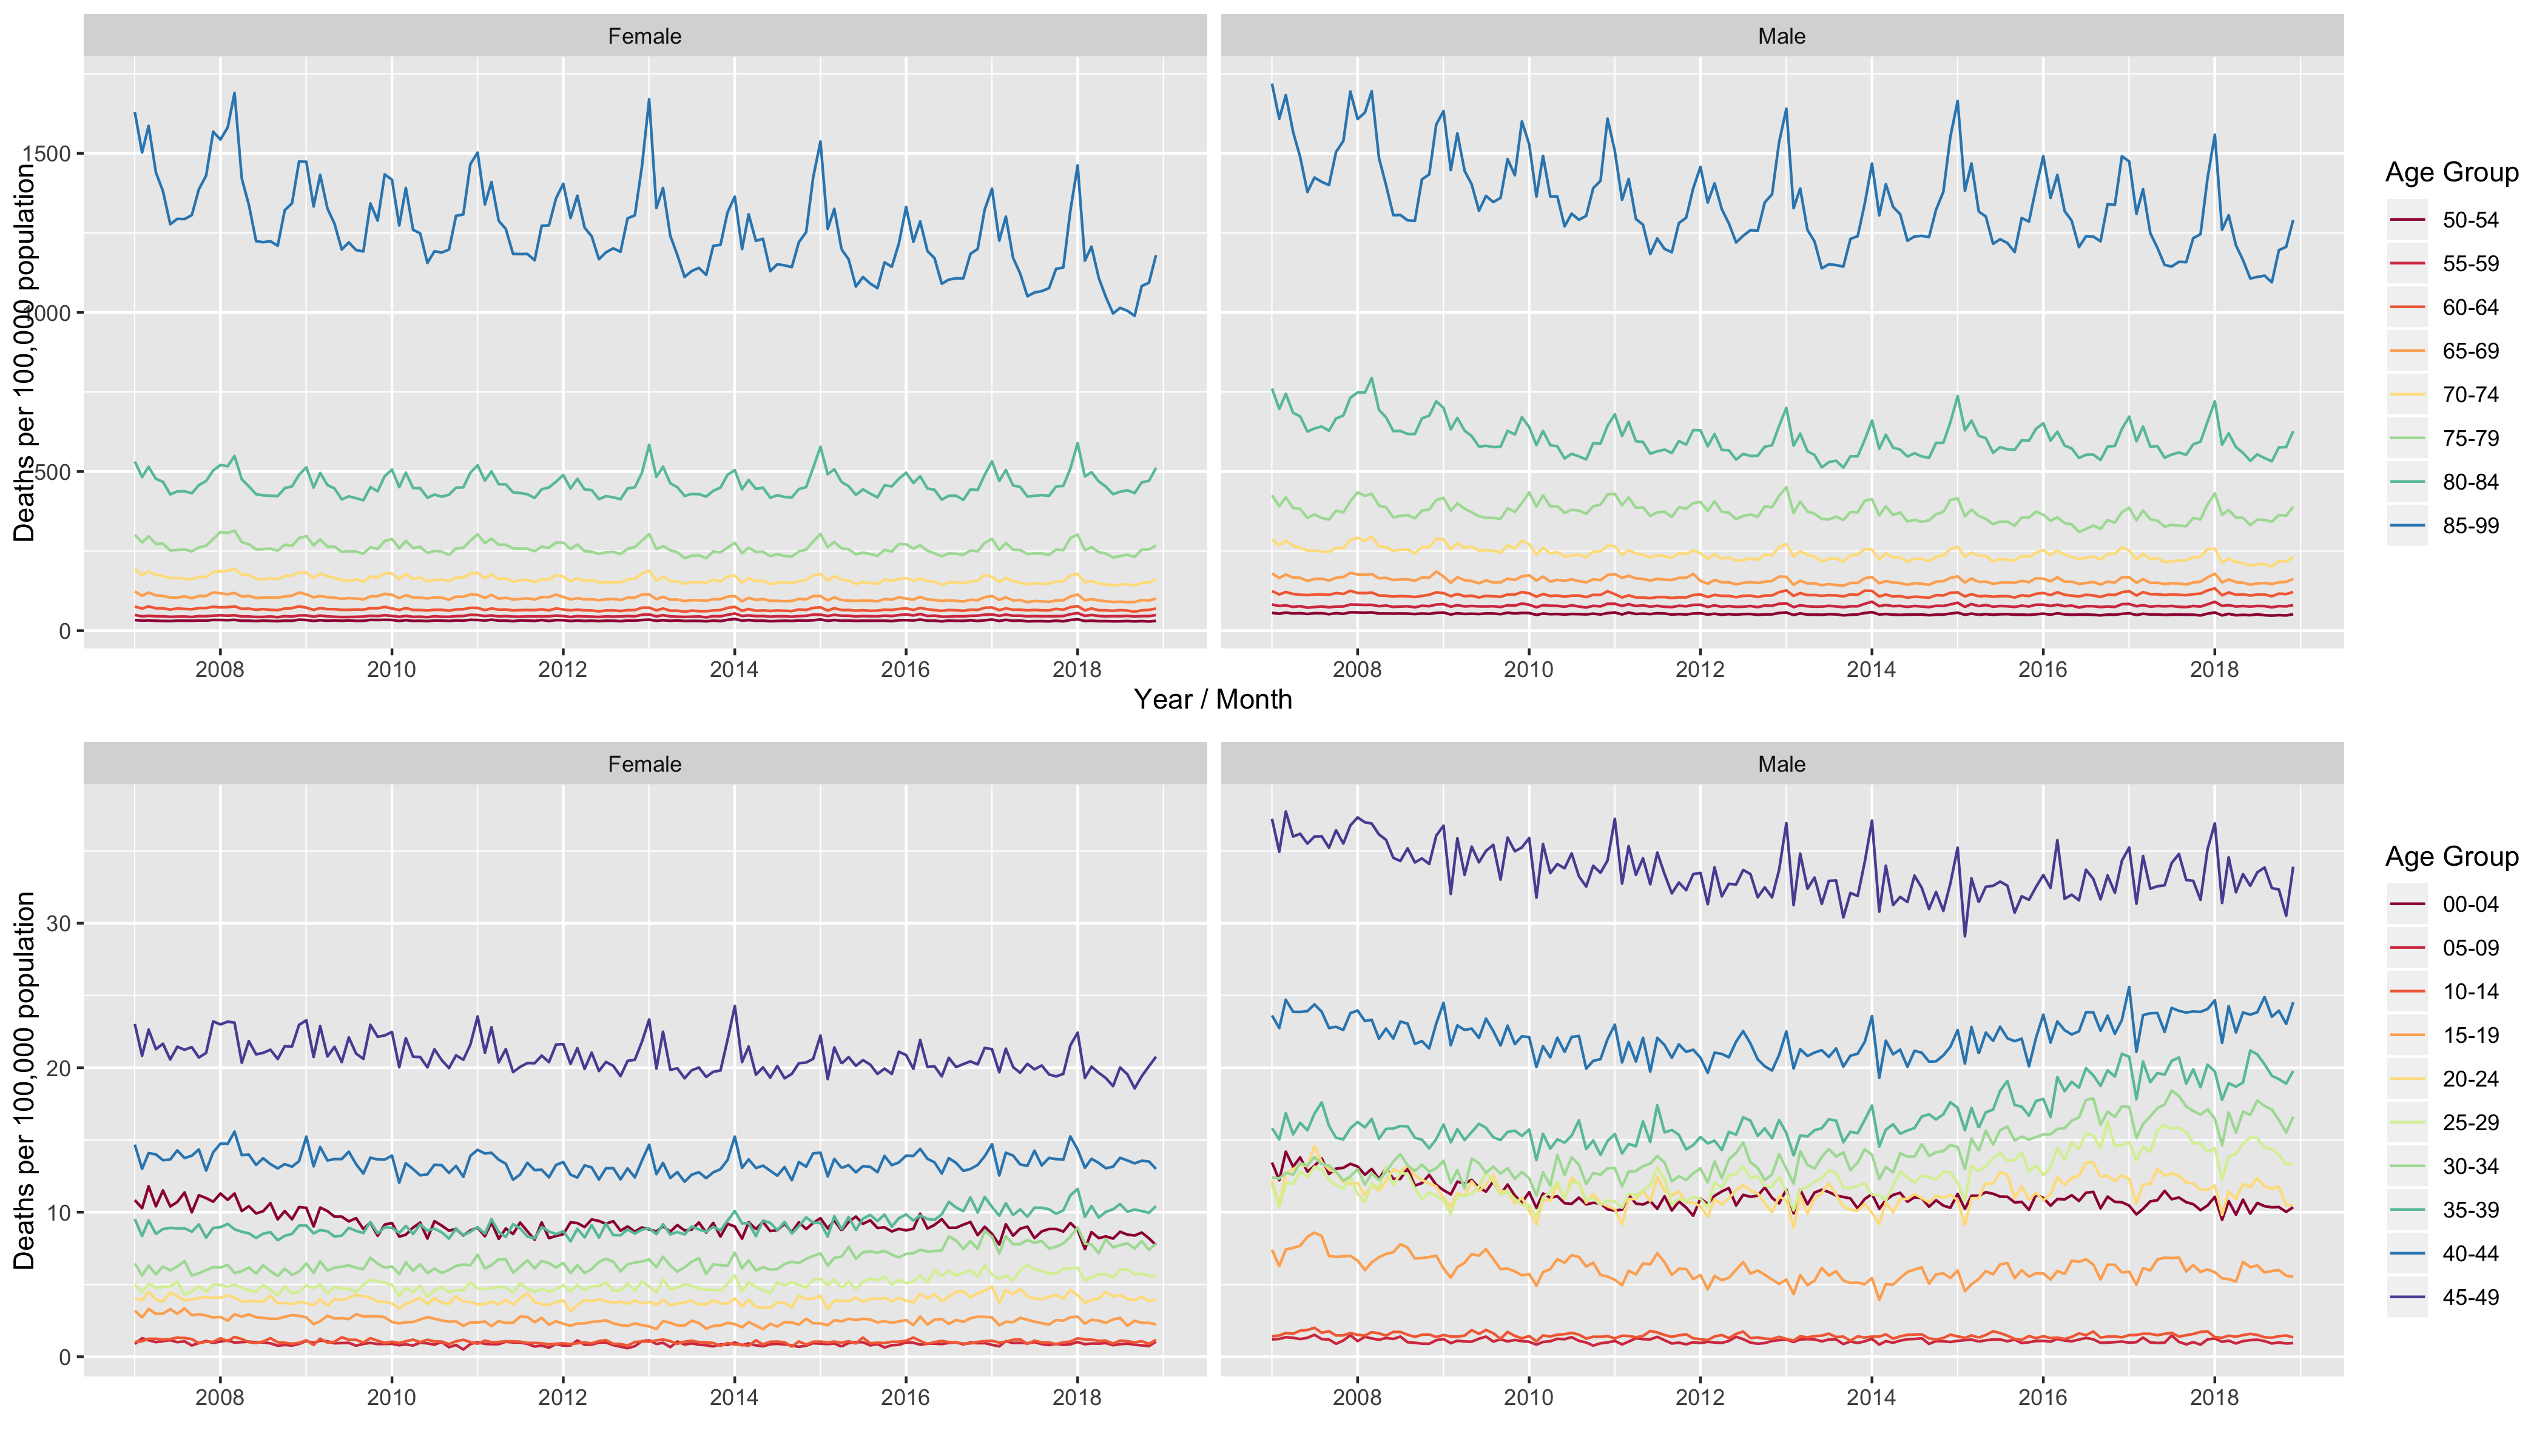
\includegraphics[width=1\textwidth, center]{../figures/eda.png}
    \caption{Trends in number of deaths per 100,000 people in the U.S. population, by year and month, sex, and age group. The plots for each gender are split into two in order to show trends for younger age groups, with the top panel showing younger age groups.}
    \label{fig:eda}
\end{figure}

As we can see in \textbf{Figure \ref{fig:eda}}, monthly mortality rate appears to vary with all of our available covariates. It appears that men tend to have higher monthly mortality rates then women (which aligns with our understanding that the life expectancy of women in the U.S. has been historically longer than men \cite{sex}). The mortality rate tends to increase with age group, except that the mortality rate for infants to toddlers (ages 0 to 4 years) is higher than the mortality rate for adolescents through young adults (ages 5 to 24 years). There is also a clear seasonal trend by month, with mortality rate the highest in January, then dipping through the summer months and rising again through October to December. There is also a relatively consistent spike down in February, and a rise again in March.

It does appear that the trends in mortality for some factors differ by other demographic variables. For instance, different age groups appear to have different patterns of mortality by year; it appears that mortality is relatively stable over the years for the 80-84 age group, but decreased for the 0-4 age group. Additionally, it appears that the impact of age differs for men and women, especially for young adults. Using linear regression, we will explore whether these trends can explain the variation in monthly mortality rate, which we describe in the following section.

\section{Explaining variability in mortality rate}

\subsection{Model selection}\label{mod.sel}

Since the distribution of mortality per 100,000 people is highly right skewed and only takes values greater than zero, we apply a log transformation to the response. Thus, when interpreting a coefficient $\beta$ for factor $X_1$, a one unit increase in $X_1$ is associated with a $e^{\beta}$ multiplicative effect on the mortality per 100,000 people.

Our first research goal is to determine the trends in mortality over time and whether these trends vary for different demographic groups, therefore we are interested in determining whether interaction terms between the time variables and sex and age explain variance in mortality rate in addition to the interaction between sex and age. Informed by the EDA, we start by fitting a full model including year, month, age group, sex, population, and interactions between sex and age, sex and month, sex and year, age and year, month and year. Since the observation is at the year/month/age group/sex level, and all but year are factor variables we are weary to include too many interaction terms since this would lead to a model where there would be essentially a different intercept for each observation.

Starting with this full model (Model 1), we remove each interaction at a time using AIC and BIC to determine whether the model with one less interaction is preferable, which is summarized in \textbf{Table \ref{tab:aic-bic}}.\footnote{The \texttt{xtable} package \cite{xtable} was used to create table and the table formatting is based on the table formatting in Daniel Kessler's applied QR, 2018.} We note that while AIC indicated a preference for keeping the interaction between year and month (comparing between Model 1 and Model 2), BIC preferred the model without (since BIC will prefer a simpler model). Since we were interested in simplifying the model, we chose to remove this interaction term, but this should not be interpreted as indicating that the monthly trend does not differ by year. We pare the model down to include year, month, age group, sex, population, and interactions between sex and age, sex and month, and age and year (Model 3 in \textbf{Table \ref{tab:aic-bic}}). The rest of this report will discuss Model 3.

\begin{table}[t]
\centering
\begingroup\tabcolsep=0.11cm\small
\begin{tabular}{lcccccrr}
 & \multicolumn{5}{c}{Interactions Included} & \multicolumn{2}{l}{} \\ \cline{2-6}
  Model & year:month & sex:year & sex:month & sex:age & age:year & \multicolumn{1}{c}{AIC} & \multicolumn{1}{c}{BIC} \\
  \hline
Model 1 & X & X & X & X & X & -12844 & -12254 \\
  Model 2 &  & X & X & X & X & -12827 & -12309 \\
  \textbf{Model 3} &  &  & \textbf{X }& \textbf{X }& \textbf{X} & \textbf{-12828} & \textbf{-12317} \\
Model 4 &  &  &  & X & X & -5575 & -5175 \\
  Model 5 &  &  & X &  & X & -12740 & -12301 \\
  Model 6 &  &  & X & X &  & -11110 & -10710 \\
   \hline
Model 7 &  &  &  &  &  & -4925 & -4709 \\
   \hline
\end{tabular}
\endgroup
\caption{AIC and BIC used for model selection. All models include year, month, age group, sex, and population as single terms and X's indicate which interaction terms are include.}
\label{tab:aic-bic}
\end{table}

Considering one-hot encoding, Model 3 includes 76 factors, which is still within reason given our sample size of over 5,000. The variables and interactions included explain almost all of the variance in mortality (with an R-squared value of .998). The residuals appear approximately normal (although with somewhat heavy tales) in a normal quantile plot and histogram (not shown here for brevity), so we are reasonably satisfied that the model assumptions are met. There are no observations with high leverage nor influence.

\subsection{Estimated effects of demographic factors on mortality}\label{ests}

Due to the number of coefficients estimated in the model, we will not present the table of coefficients, but rather visualize or describe the effect of each covariate. Most coefficients are significant at the 5\% level, and we indicate whether estimated coefficients are significant when relevant. As mentioned in \textbf{Section \ref{mod.sel}}, all effects shown are multiplicative effects, so an effect greater than 1 indicates increased mortality while an effect between 0 and 1 indicates decreased mortality. In this discussion it is assumed that all other variables, other than those directly discussed, are held constant.

The coefficient for population is significant, however we don't estimate a practical effect of population on mortality rate, with a one thousand person increase in population associated with a .999 multiplicative effect on the mortality per 100,000 people. Thus, as the population increases, holding all other variables constant, our model estimates a slight decrease in the mortality rate.

\begin{figure}[ht]
    \centering
   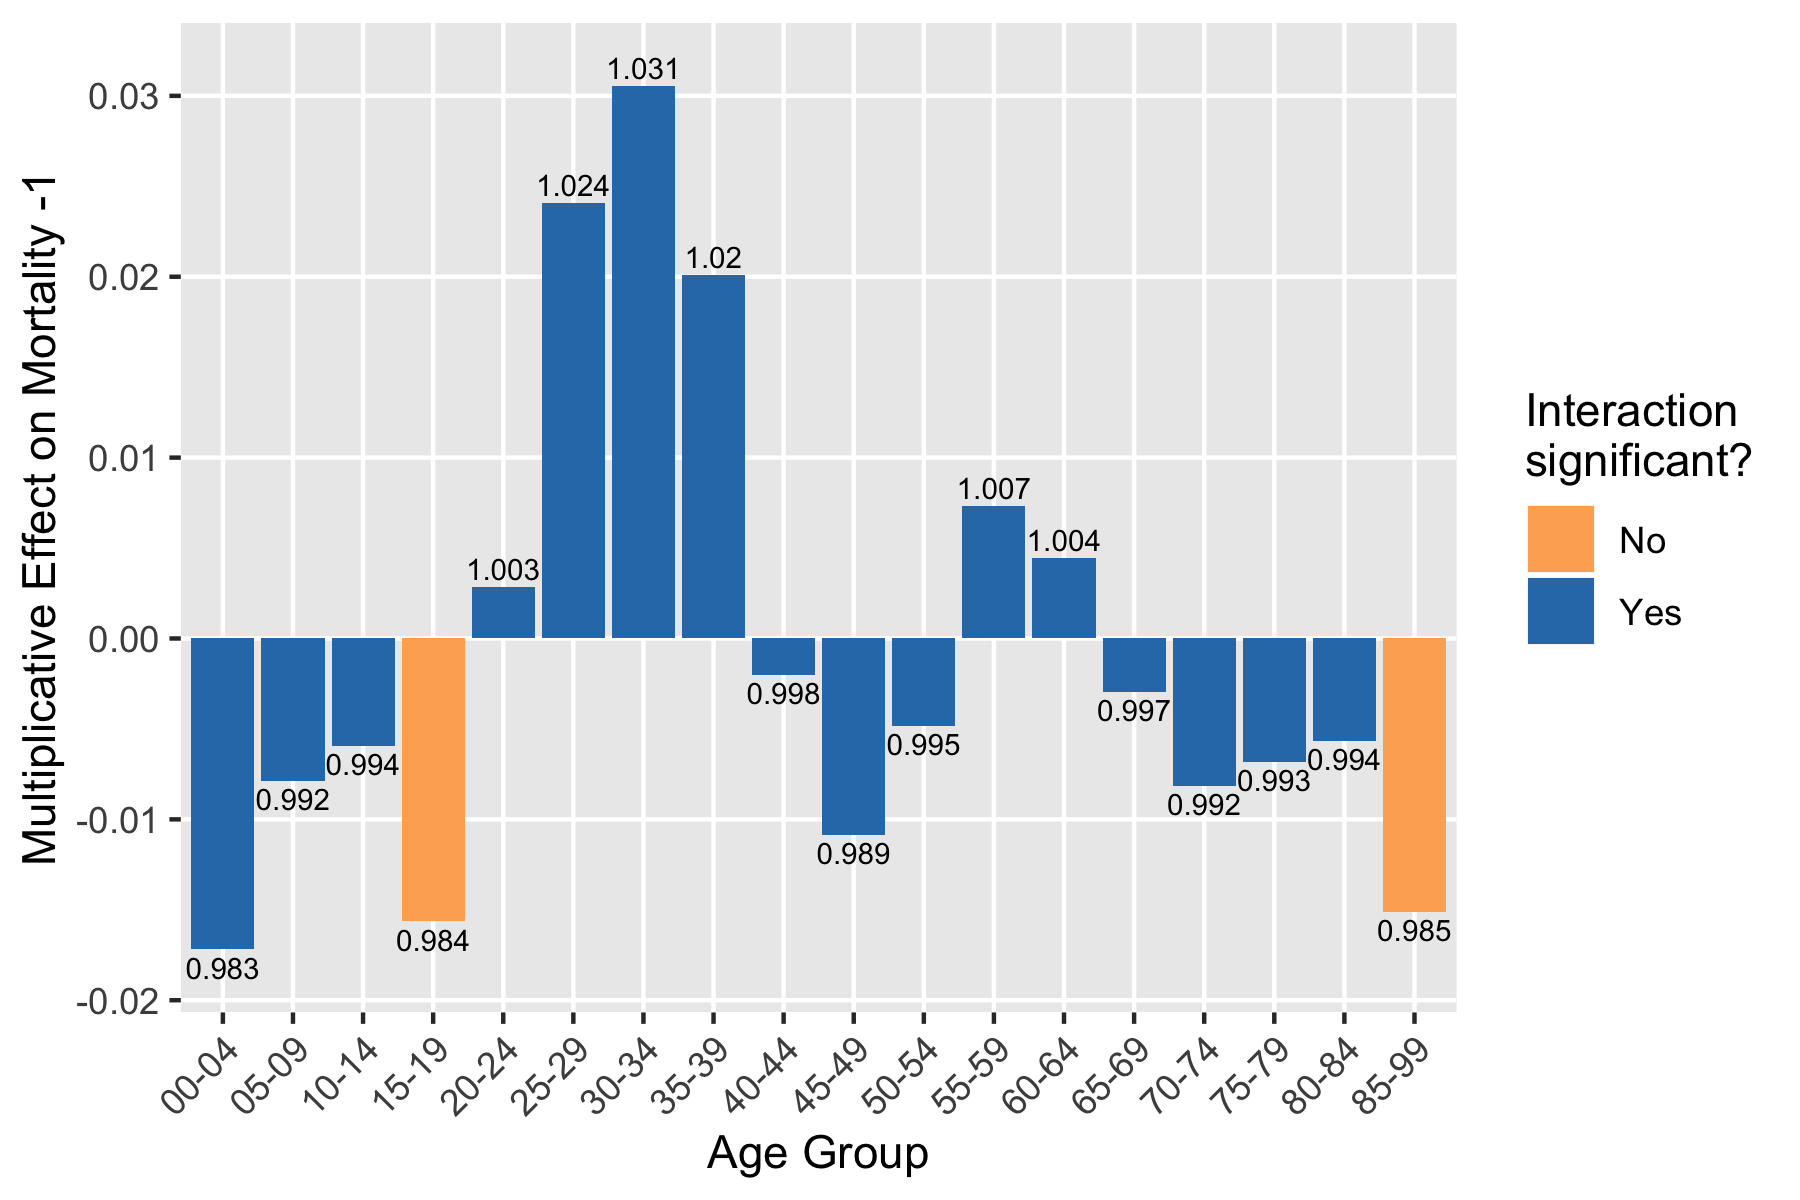
\includegraphics[width = .6\textwidth]{../figures/year_effect.png}
       \caption{Multiplicative effect of one year increase on mortality - 1 by age group. The actual multiplicative effect is included in text above bars. One is subtracted from the multiplicative effect for this plot in order to show more contrast in the effect of year between different age groups. A negative bar indicates that the multiplicative effect is between 0 and 1, while a positive bar indicates that the multiplicative effect is greater than 1.}
         \label{fig:year_eff}
\end{figure}

As shown in\textbf{ Figure \ref{fig:year_eff}}, the effect of a one year increase on mortality rate differs by age group, holding all else constant. The model estimates that mortality decreased for U.S. residents 19 years or younger, 40-54 years, and 65 years and older and mortality increased for U.S. residents between the ages of 20-39 and 55-64 each year over the time period 2007-2018. Note however, that the multiplicative effect is not large (for 30-34 year old adults, a one year increase is associated with a 1.03 multiplicative effect on mortality rate, holding all else constant, for example). We estimate that a one year increase was most beneficial in decreasing mortality for infants and toddlers in the U.S., with an estimated multiplicative effect of around .98.

From \textbf{Figure \ref{fig:month_eff}} we can see that compared with January, all other months have a multiplicative effect of less than 1 on mortality (in other words we estimate that mortality is lower in these months than in January). There isn't a consistent curved trend, but in general for women, being in the months of June-September have the largest reductive effect on mortality compared with January. This trend doesn't hold for men. The model picks up the drop in mortality between January and February and then spike up in March that we noticed in our EDA (See \textbf{Section \ref{eda}}).

\begin{figure}[ht]
    \centering
   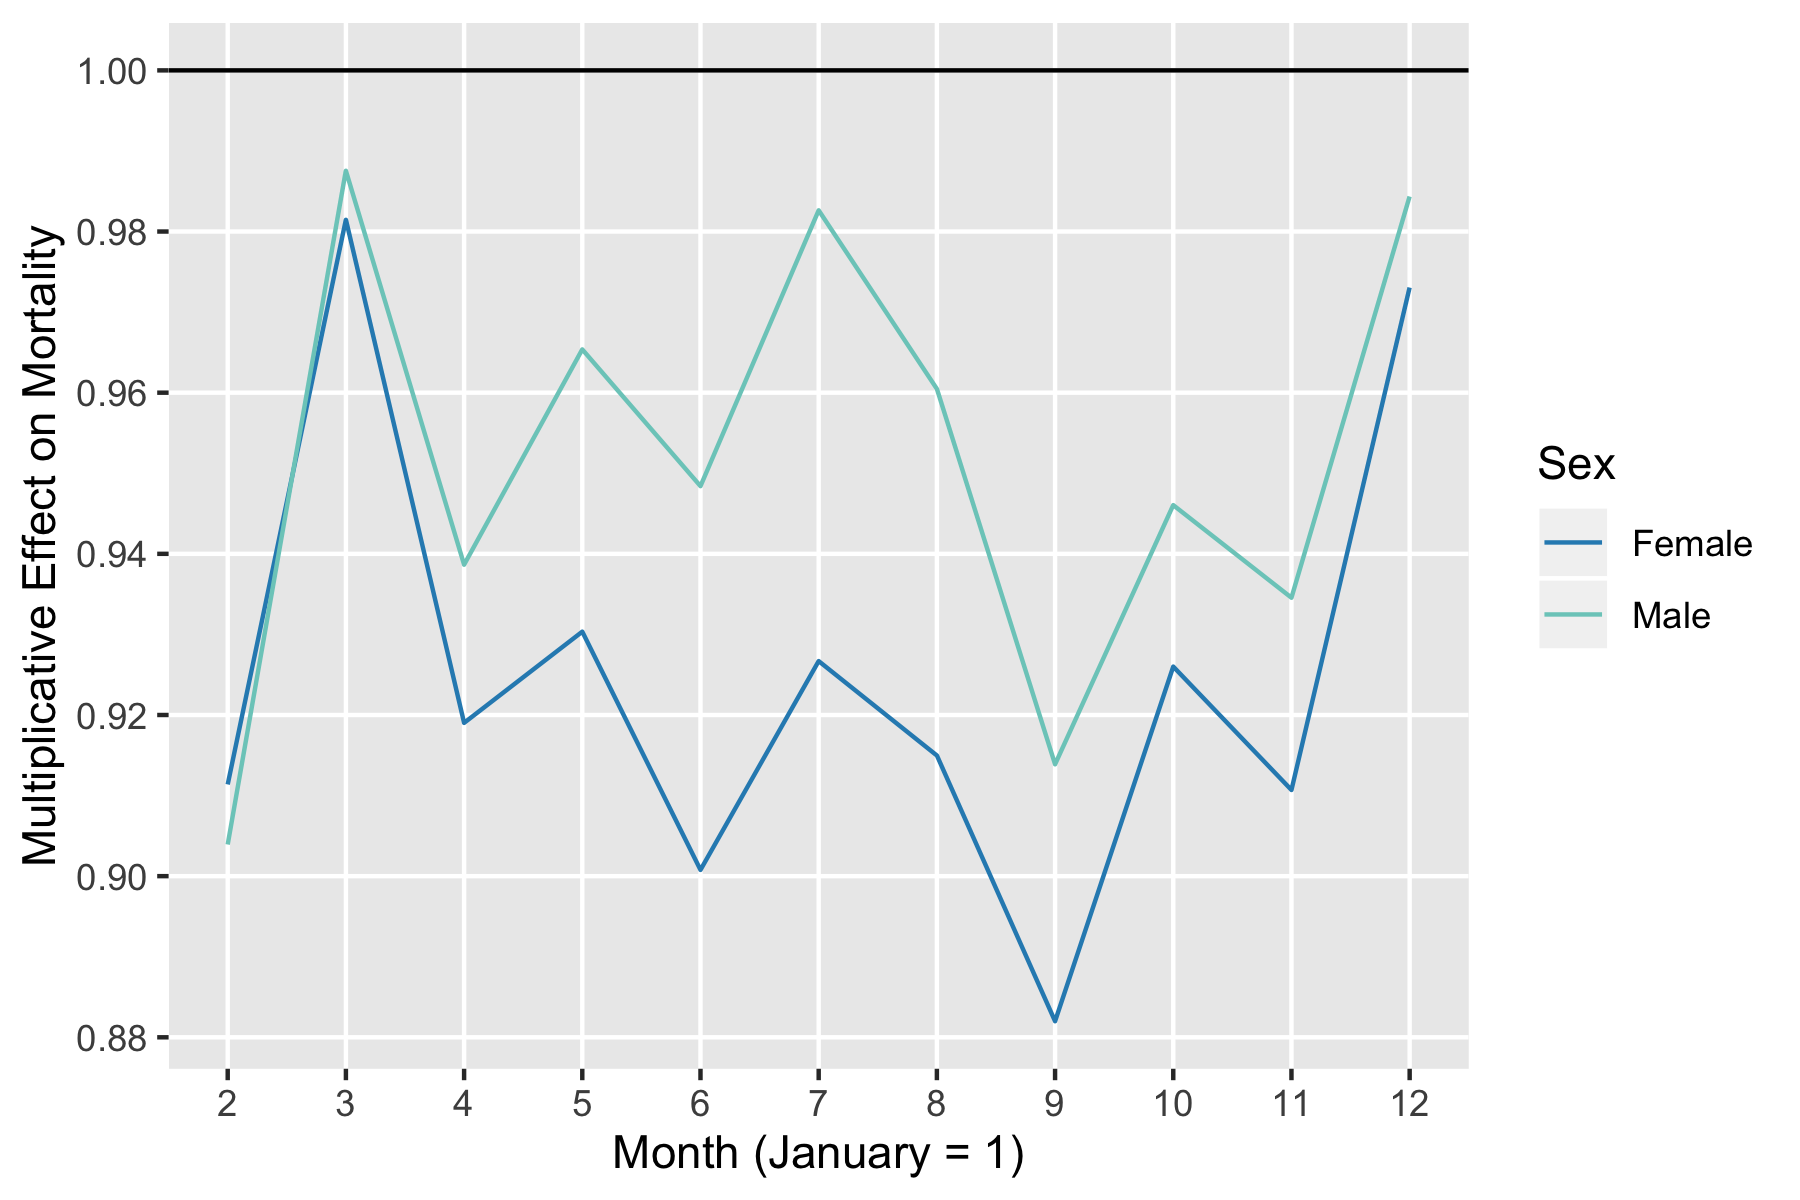
\includegraphics[width = .6\textwidth]{../figures/month_effect.png}
   \caption{Multiplicative effect on mortality of each month, as compared to January, for males and females. The interaction term between sex and month is not significant for February, March, and December. Each estimated coefficient for month is significant.}
         \label{fig:month_eff}
\end{figure}

\begin{figure}[ht]
    \centering
    \makebox[\linewidth][c]{%
    \begin{subfigure}[t]{0.5\textwidth}
        \centering
        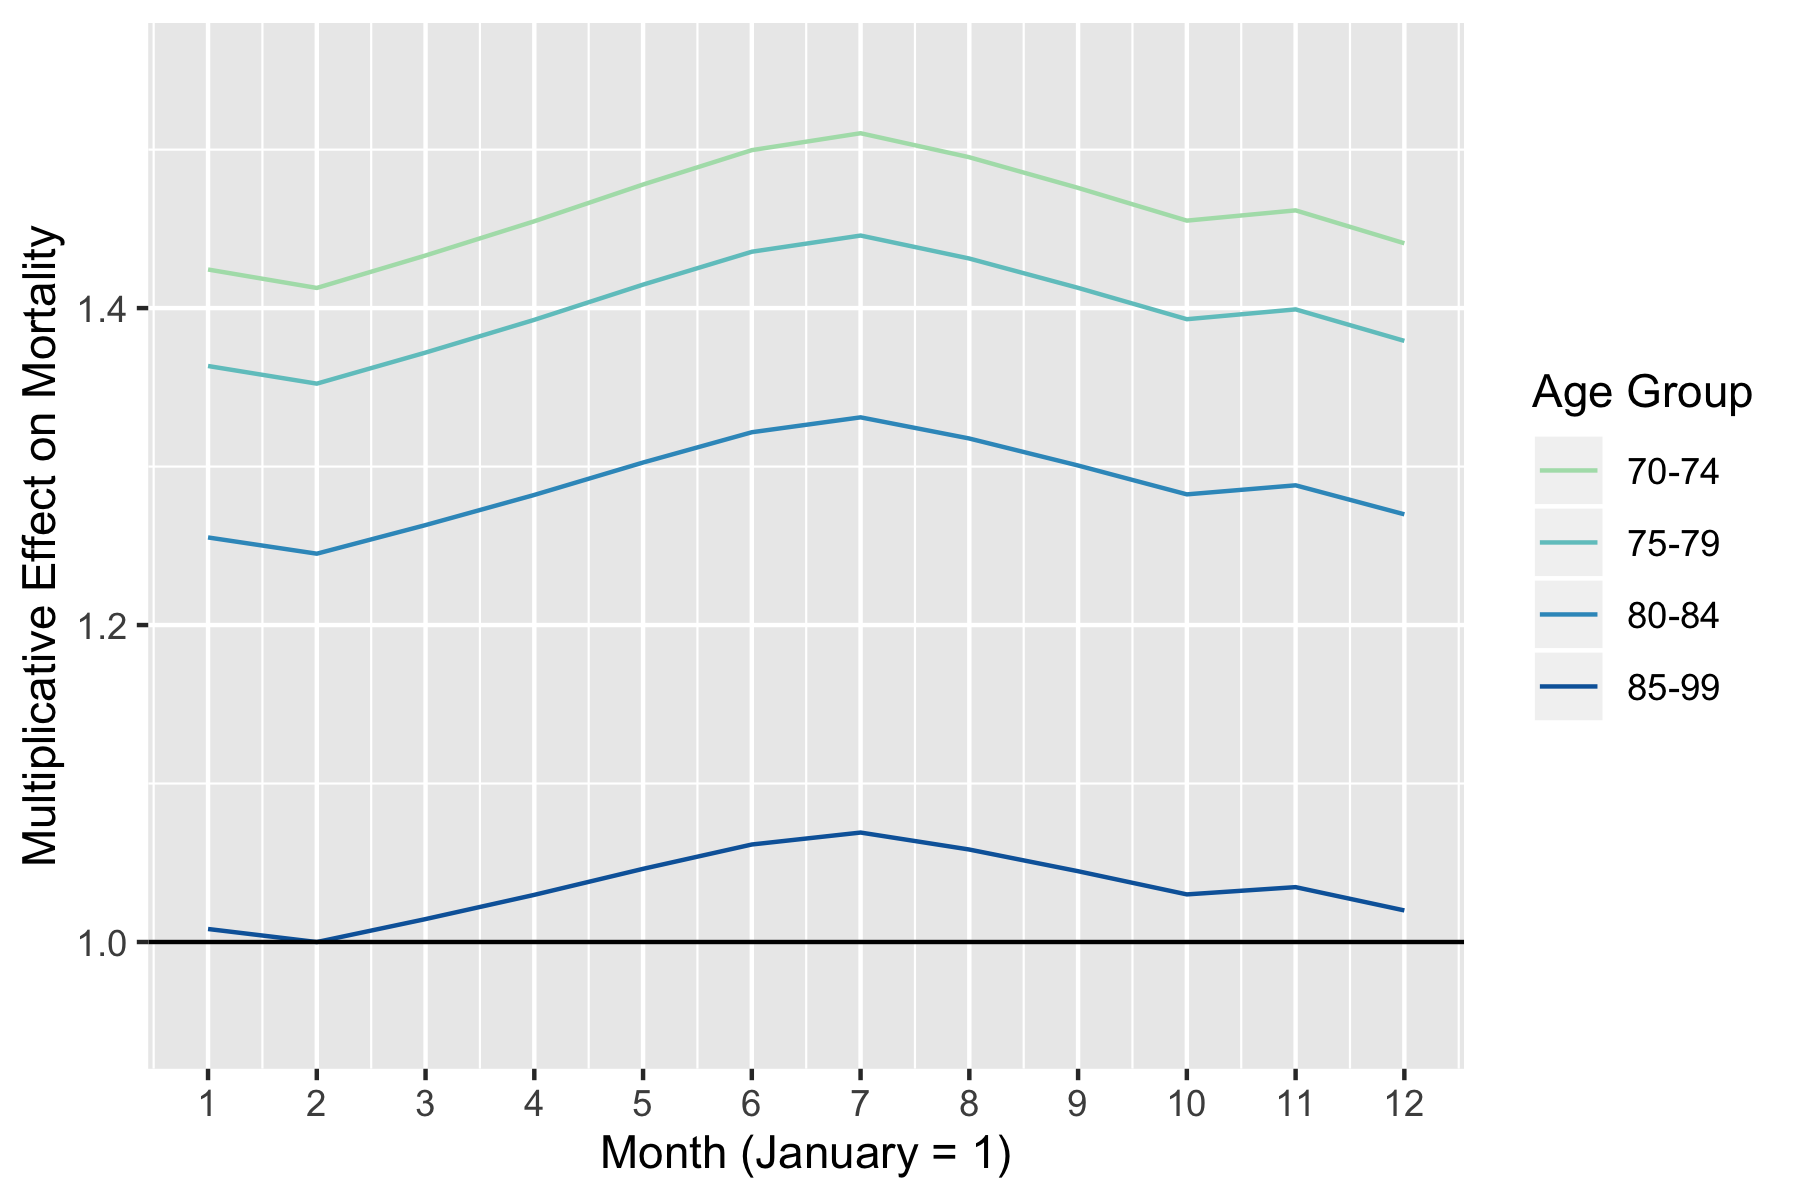
\includegraphics[width = \textwidth]{../figures/gender_effect_month.png}
        \caption{Multiplicative effect of being male (as compared with female) and in different months on monthly mortality rate for U.S. residents age 70 and older. The interaction term between sex and month is not significant for February, March, and December.}
         \label{fig:gend_month_eff}
    \end{subfigure}\hspace{0.02\textwidth}%
    \begin{subfigure}[t]{0.5\textwidth}
        \centering
        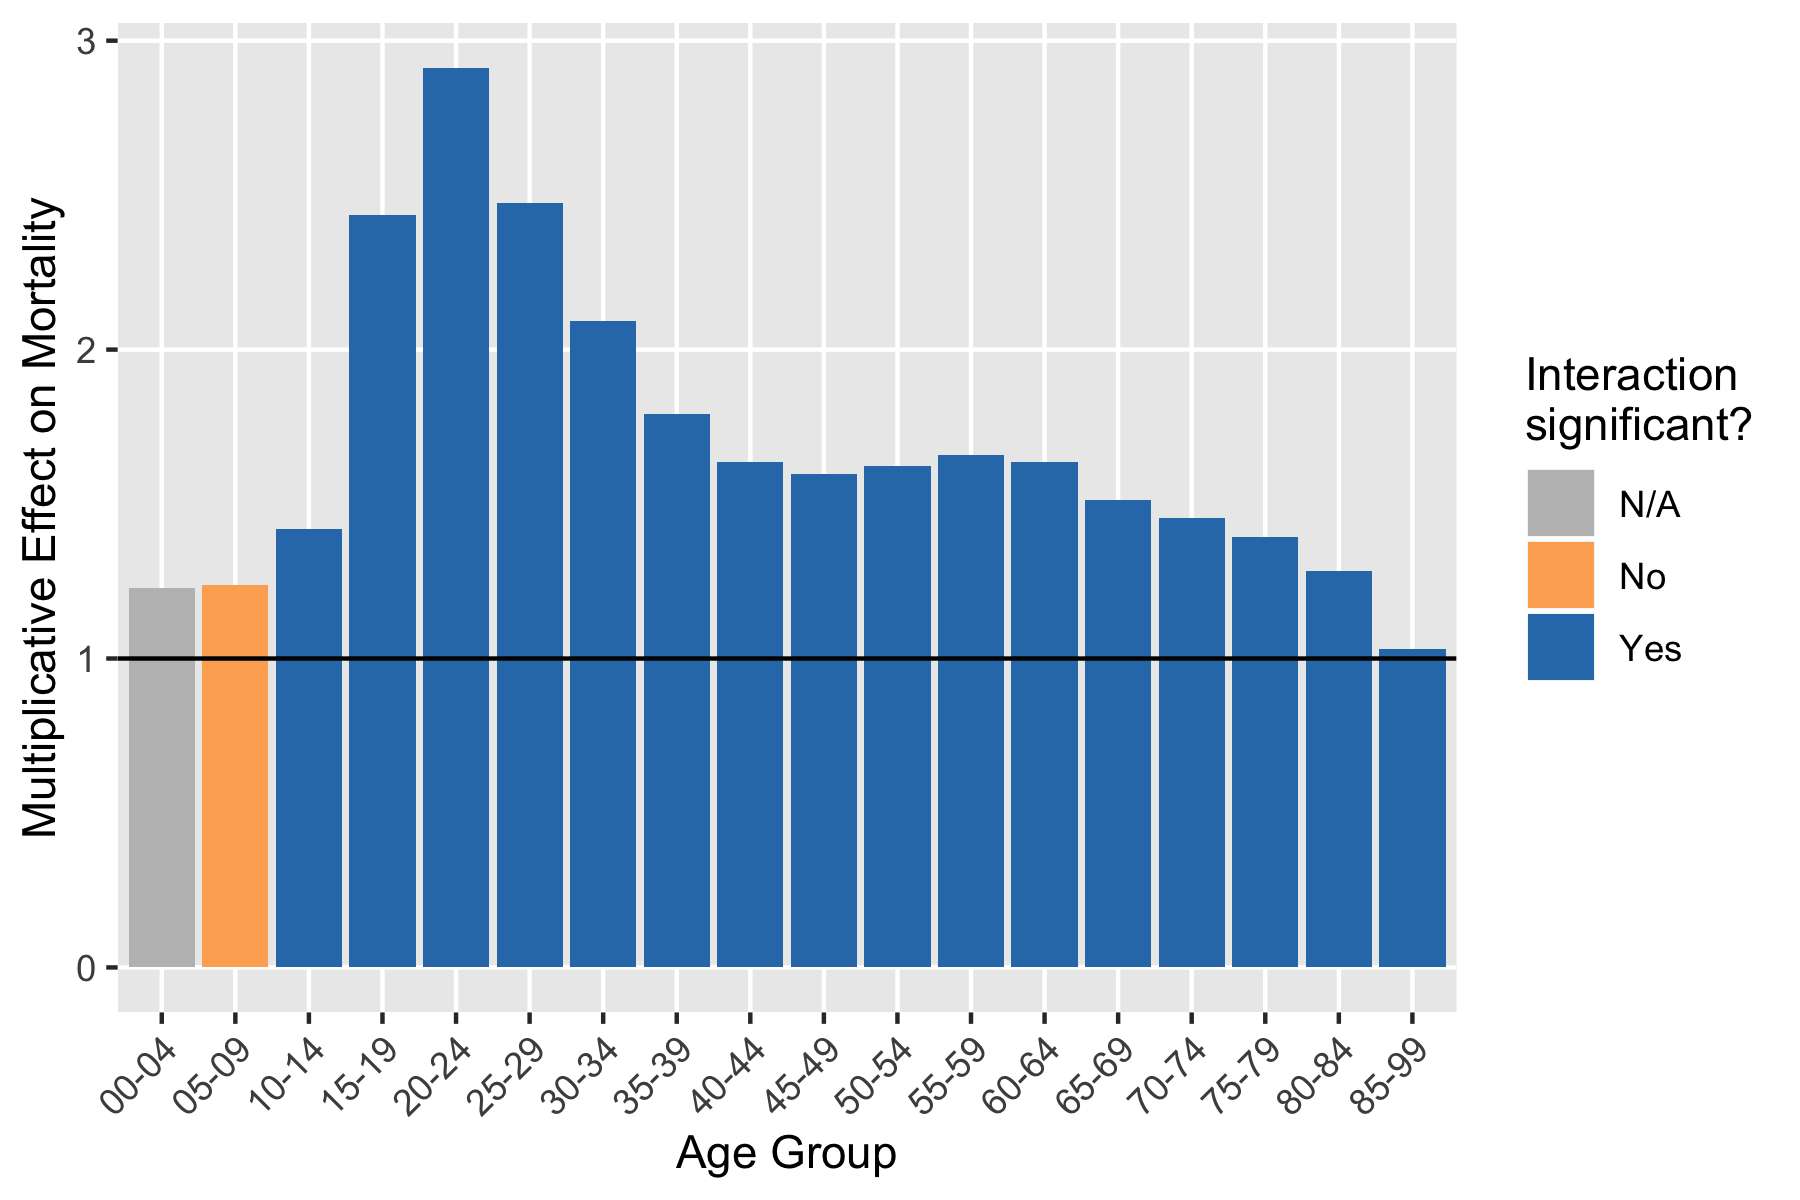
\includegraphics[width = \textwidth]{../figures/gender_effect_age1.png}
         \caption{Multiplicative effect of being male (as compared with female) and in different age groups on monthly mortality rate, for the month of October. Other months have a similar trend.}
         \label{fig:gend_age_eff}
    \end{subfigure}
    }
     \caption{Multiplicative effect of sex on mortality per 100,000 people by month and age group.}
\end{figure}

\begin{figure}[ht]
    \centering
    \makebox[\linewidth][c]{%
    \begin{subfigure}[t]{0.5\textwidth}
        \centering
        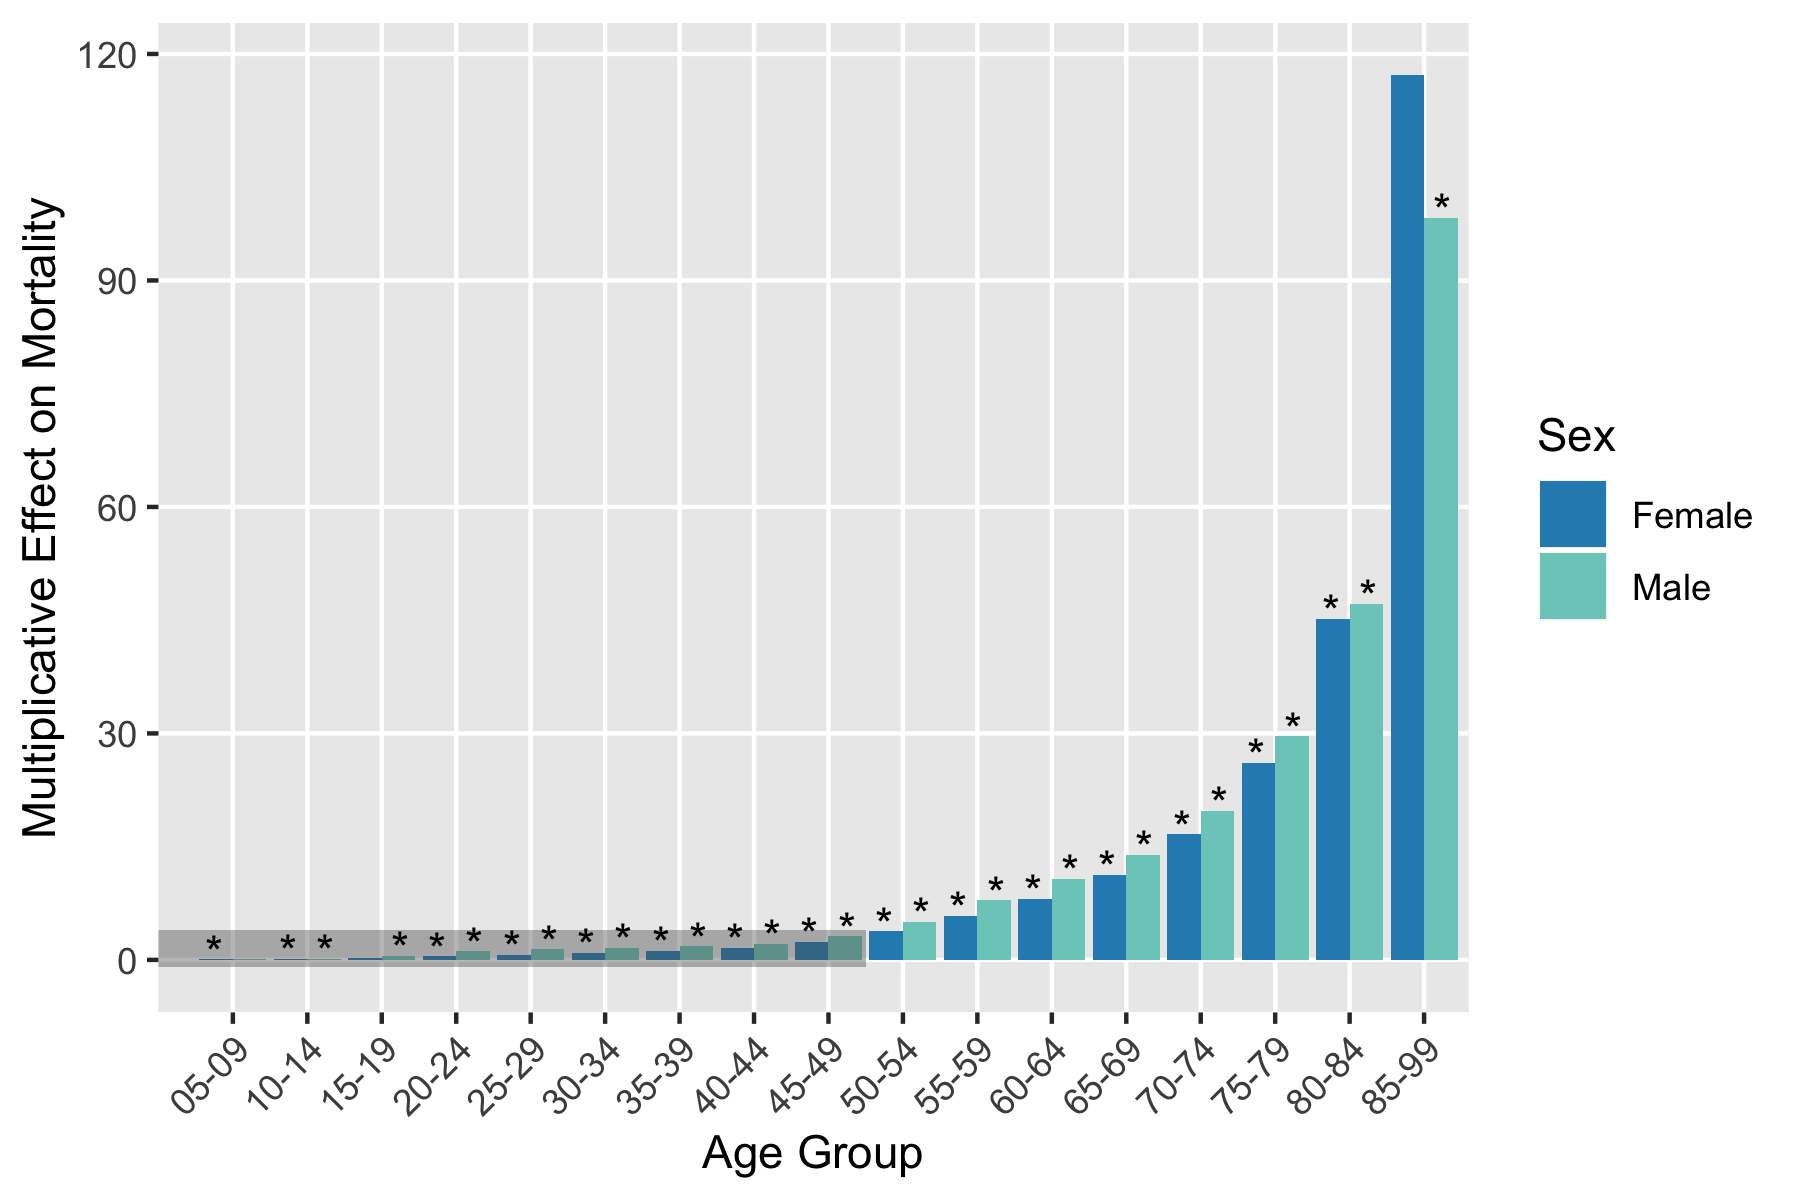
\includegraphics[width = \textwidth]{../figures/age_effect_all.png}
        \caption{Multiplicative effect of each age group (as compared with age group 0-4 years) and for the two sexes on monthly mortality rate. The plot area shaded in grey is shown in the figure to the right (Figure 5b).}
         \label{fig:age_eff}
    \end{subfigure}\hspace{0.02\textwidth}%
    \begin{subfigure}[t]{0.5\textwidth}
        \centering
        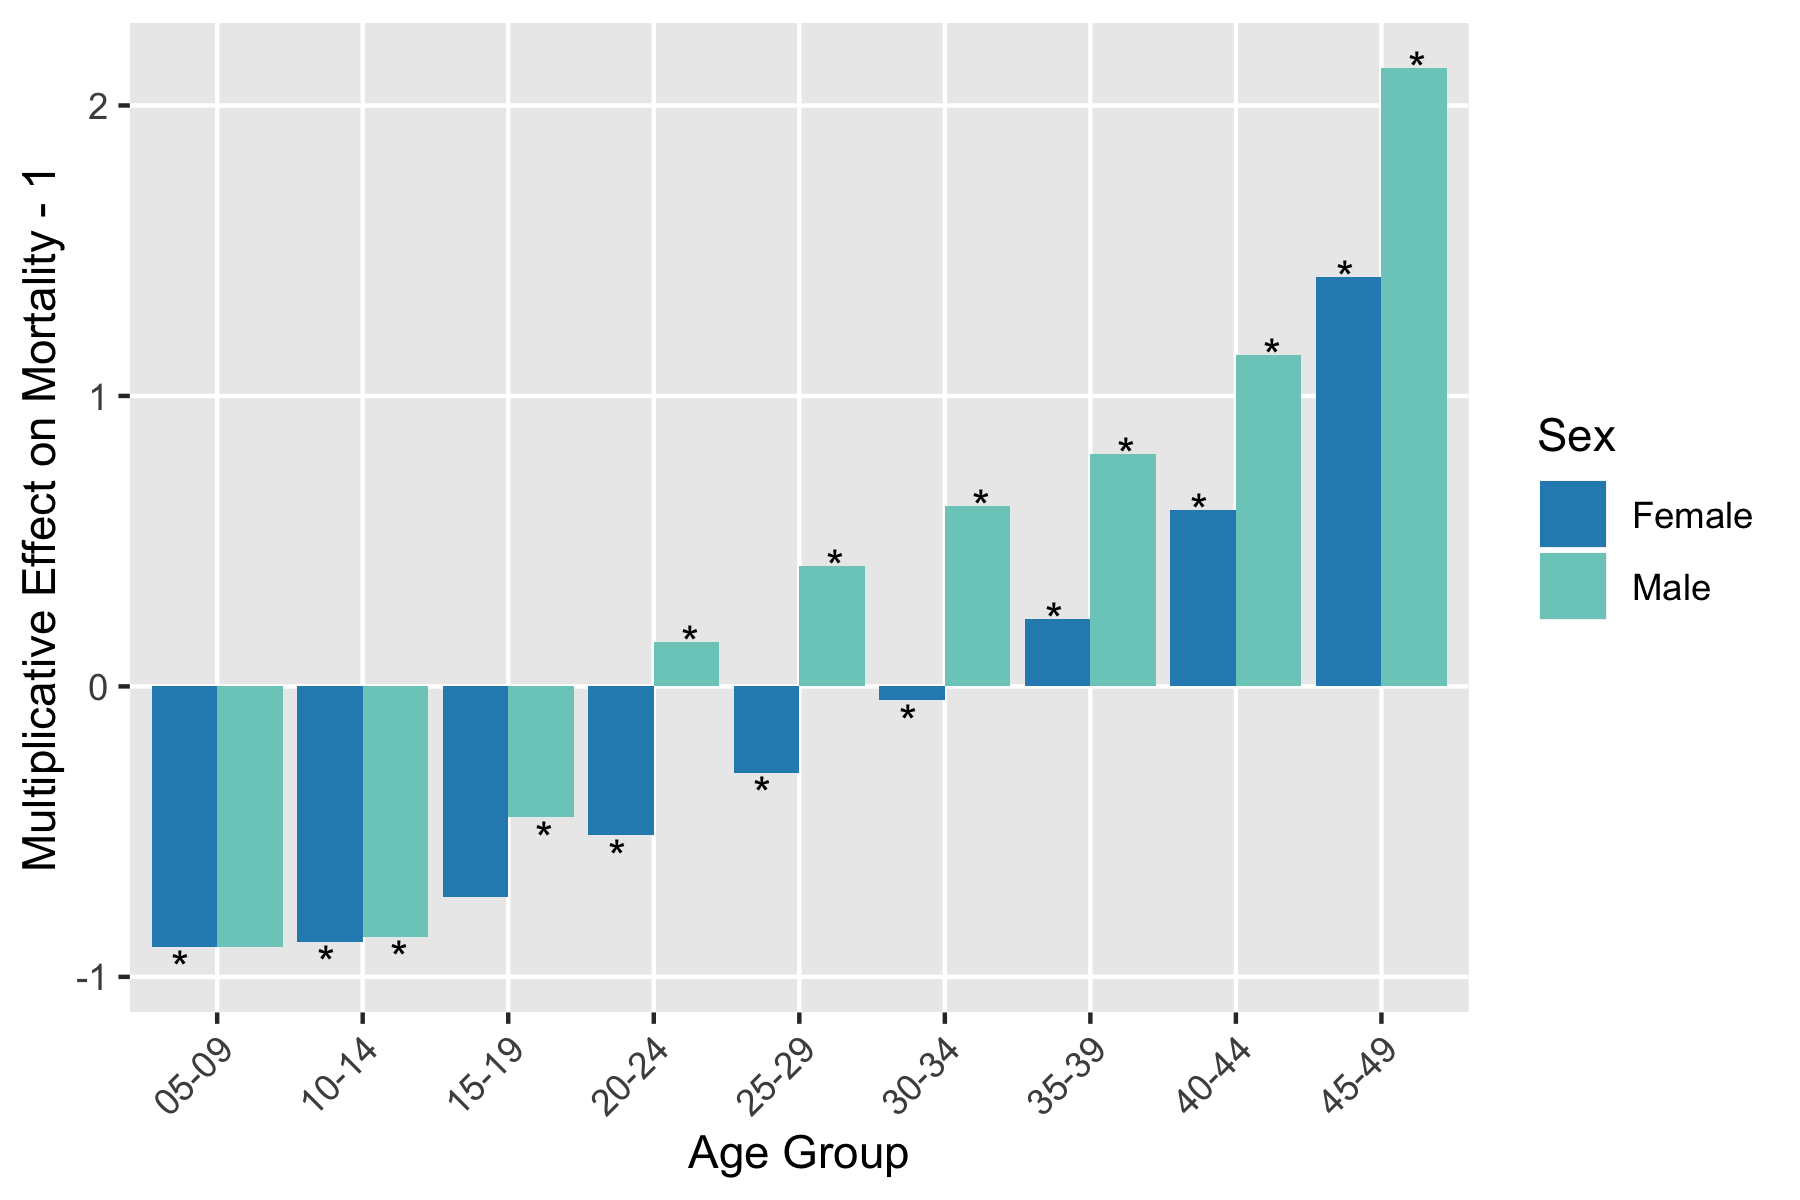
\includegraphics[width = \textwidth]{../figures/age_effect_young2.png}
         \caption{Multiplicative effect - 1 of each age group (as compared with age group 0-4 years) and for the two sexes on monthly mortality rate for ages 5 to 49 years. See Figure 2a for detailed explanation of interpretation for negative versus positive bars.}
         \label{fig:age_effyoung}
    \end{subfigure}
    }
     \caption{Multiplicative effect of age on mortality per 100,000 people by sex for 2018. Stars above the effect for females indicate a significant coefficient for that age group and stars above the effect for males indicate a significant coefficient for the interaction between sex and that age group.}
\end{figure}

\textbf{Figures \ref{fig:gend_month_eff}} and \textbf{\ref{fig:gend_age_eff}} show the estimated effects of being male as compared with being female on monthly mortality, by month and age group (which we felt was best illustrated separately). We estimate that the multiplicative effect of being male on mortality is always greater than 1 (which again aligns with our general understanding of life expectancy and our EDA). \textbf{Figure \ref{fig:gend_month_eff}} illustrates the estimated multiplicative effect on mortality of being male and in certain months for U.S. residents above age 70. These age groups are shown as examples as the trend in the effect of sex by month are similar for all age groups. \textbf{Figure \ref{fig:gend_month_eff}} shows that being male has a the greatest estimated multiplicative effect on mortality for the summer months, June - August. This aligns with the trend shown in \textbf{Figure \ref{fig:month_eff}}. \textbf{Figure \ref{fig:gend_age_eff}} shows the multiplicative effect on mortality of being male and in each age group, for the month of October. We chose to show only one month for easier illustration since the trend by age is similar for all other months. We estimate that the disparity between male and female mortality is the greatest for teens through young adults (ages 15 to 24), with an estimated mortality rate of 2 to 3 times larger for males than for females, and is the lowest for the elderly (ages 85 to 99) and children (ages 0 to 9).




Finally, we consider the estimated effect of age group on monthly mortality. \textbf{Figure \ref{fig:age_eff}} shows the estimated multiplicative effect of each age group as compared to the age group 0-4 years in 2018, and how this effect differs for males and females. \textbf{Figure \ref{fig:age_effyoung}} shows the same but for ages 5-49 so that the patterns are easier to see for the younger age groups. These two figures illustrate that as compared to the 0-4 year age group, being in age groups for ages over 35 has a multiplicative effect greater than 1 and this effect increases as age increases. The effect of being in the 85-99 group is greater for females than for males. In 2018, the estimated mortality rate is greater for men in their 20s to 30s than male infants, but the estimated mortality rate is less for females in their 20s to 30s than female infants. Finally, we estimate that just by reaching five years of age and through 19 years of age, the mortality rate is around 10\% to half of the mortality for 0-4 year old children for both females and males in the US. As shown in \textbf{Figure \ref{fig:year_eff}}, the model estimates different effects of year for different age groups. While the trends shown in \textbf{Figure \ref{fig:age_eff}} and \textbf{Figure \ref{fig:age_effyoung}} generally hold for earlier years, for years 2007-2009, the estimated mortality rate is \textit{lower} for men in their 20s to 30s than male infants.

In summary, we found that there appears to be a seasonal effect, month by month on mortality, but that differs by gender, and there appears to have been an effect over time (years) on mortality rate, but that differs by age group. In addition, we estimate that being male is associated with higher mortality, but that the magnitude of the effect of being male depends on month and age group. Finally, age has a clear effect on mortality rates, with the greatest multiplicative effects for old ages as compared to infants, and the effect of age differs by sex.

\section{Predicting mortality rate}

\subsection{Methodology}

In order to determine how well we can predict the number of deaths per 100,000 people for different demographic groups and over time, we compare the linear model to three more models: a Generalized Linear Model, random forest model, and gradient boosted model. A random sample of 80\% of the data is used as a training set and the other 20\% is reserved as a test set. Five-fold cross validation with the training set is used for all parameter tuning.

\subsubsection{Generalized Linear Model}

Since the number of deaths per 100,000 people is a value restricted above 0, rather than using a linear model with a log transformed response, it makes sense fit a Generalized Linear Model (GLM) with a Gaussian family and log link function, which we fit with the same variables and interactions as the linear model. We will refer to this model as ``GLM" for the remainder of the report and the original multiple linear regression model as the ``linear" model, recognizing that the linear model is also a Gaussian family GLM.

\subsubsection{Random Forest and Gradient Boosting}

As another point of comparison, we fit two non-linear models to predict mortality rate, a random forest model and a tree model using gradient boosting.\footnote{The \texttt{Random Forest} and \texttt{gbm} packages are used to fit the random forest and gradient boosted models respectively \cite{gbm} \cite{randomForest}. We fit both of these models, since we expect gradient boosting may result in a lower mean squared error than the random forest model, since all variables are used at every split to grow a tree (and we know from our linear model that the interactions between variables are important), however random forest models are more resistant to overfitting.} These models may also be preferable to the two linear models we fit since they do not rely on assumptions regarding the conditional expectation or variance of the data.   By virtue of how tree-based methods work, they take into account interactions between variables, so we do not explicitly specify interactions in these models.

Since the mortality rate is highly skewed, we apply a log transformation to the response when fitting the tree-based models. Since gradient boosting relies on a squared error loss, if we do not apply the log transformation, we expect the model would favor predicting instances of high mortality over low mortality since the squared error would tend to be larger for observations with higher mortality, just by virtue of the mortality value already being large.

We tune two parameters for the random forest models: the number of variables to sample at each tree node (\texttt{mtry}), and the number of trees to grow (\texttt{ntree}). We vary \texttt{mtry} from 1 to 4 (since we only have 5 factors) and \texttt{ntree} from 75 to 600 trees at different increments (75, 100, 125, 150, 175, 200, 300, 500, and 600 trees). We find that sampling 3 variables at each node and growing 150 trees has the lowest mean squared error and avoids overfitting.

We also tune two parameters for the gradient boosting models: the ``interaction depth," or number of variable interactions allowed (\texttt{interaction.depth}), and the number of trees grown (\texttt{n.trees}). We vary \texttt{interaction.depth} from 1 to 5 and \texttt{n.trees} the same as for the random forest model. With our learning rate (\texttt{shrinkage}) as 1, we choose an interaction depth of 2 (which means that at most 2-way interactions are allowed) and to grow 300 trees.

\subsection{Model comparison}

After tuning our models using the training set, we calculate training and testing mean squared error (MSE) for each model, which are reported in \textbf{Figure \ref{fig:mod_err2}}. Using MSE as our measure of accuracy, we find that the linear model (using a log transformed response) performs by far the worst in predicting mortality. The GLM, random forest, and gradient boosted models perform similarly in terms of the training error, however, the random forest and GLM models have the smallest testing error. It seems unusual to have testing errors so much lower than the training errors, but we expect this is due to mortality being so right skewed, so having a couple observations for which high mortality aren't well predicted in the training set would lead to a higher MSE than in the test set.\footnote{We were curious about indications of overfitting, since we fit quite rich models, so we also calculated average training and testing MSE values for each model, averaging over five 80/20 test/train splits (in other words, using five-fold cross validation with the whole dataset), and found evidence of overfitting for the GLM and gradient boosting models. We are hesitant to use these averaged MSE values to make any conclusions since the original training set, used to tune the parameters are mixed up and included in these test sets.} The MSE values indicate reasonable accuracy of prediction for the GLM, random forest, and gradient boosted models considering the range and scale of mortality per 100,000 population.

\begin{figure}[ht]
    \centering
    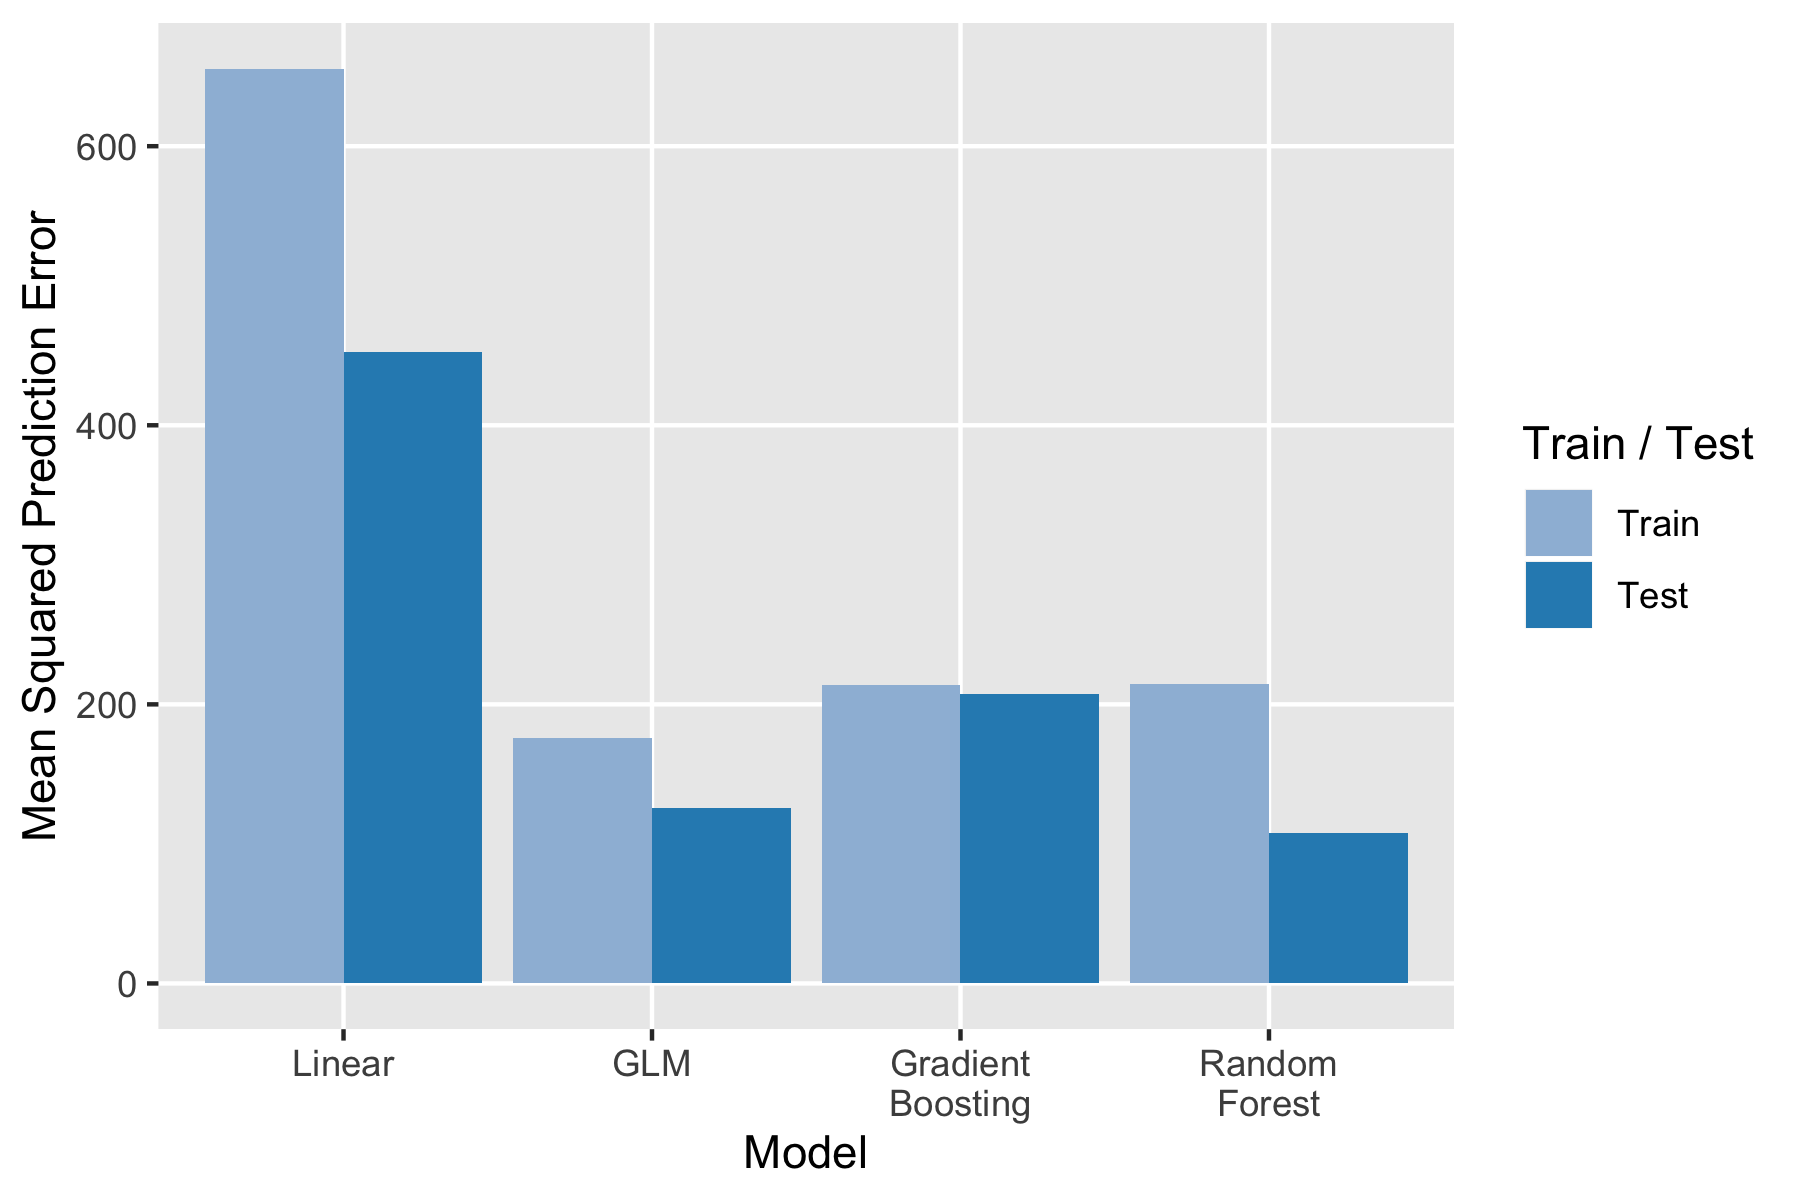
\includegraphics[width = .5\textwidth]{../figures/mod_errs2.png}
    \caption{Testing and training mean squared error for prediction models.}
    \label{fig:mod_err2}
\end{figure}

Considering practical issues other than accuracy, all of these methods have nice interpretations; for the linear regression and GLM, you can perform inference on the coefficients, as we did in Section \ref{ests} for the linear model,\footnote{The conclusions based on the coefficients of the GLM align with the linear model for almost all groups. The only distinction is that the GLM estimates that being Male reduces mortality multiplicatively, for those in the 85-99 year age group.} and for the tree-based methods, we can evaluate the variable importance.\footnote{For the regression random forest and gradient boosting models, variable importance is measured as a mean decrease in MSE and standardized to show relatively rates between variables.} As we can see in \textbf{Figures \ref{fig:vi_rf}} and \textbf{\ref{fig:vi_gb}}, the variable importance differs somewhat between the random forest and gradient boosting models, although age group is the most important. Year and month are found to have low importance in both models. The biggest distinction is that the random forest model finds population to have relative importance, which may be due to the fact that a subset of the factors are randomly selected at each node when growing a tree and so in subsets where another important variable is not present, population may have a greater effect. This warrants future investigation.

\begin{figure}[ht]
    \centering
    \makebox[\linewidth][c]{%
    \begin{subfigure}[t]{0.5\textwidth}
        \centering
        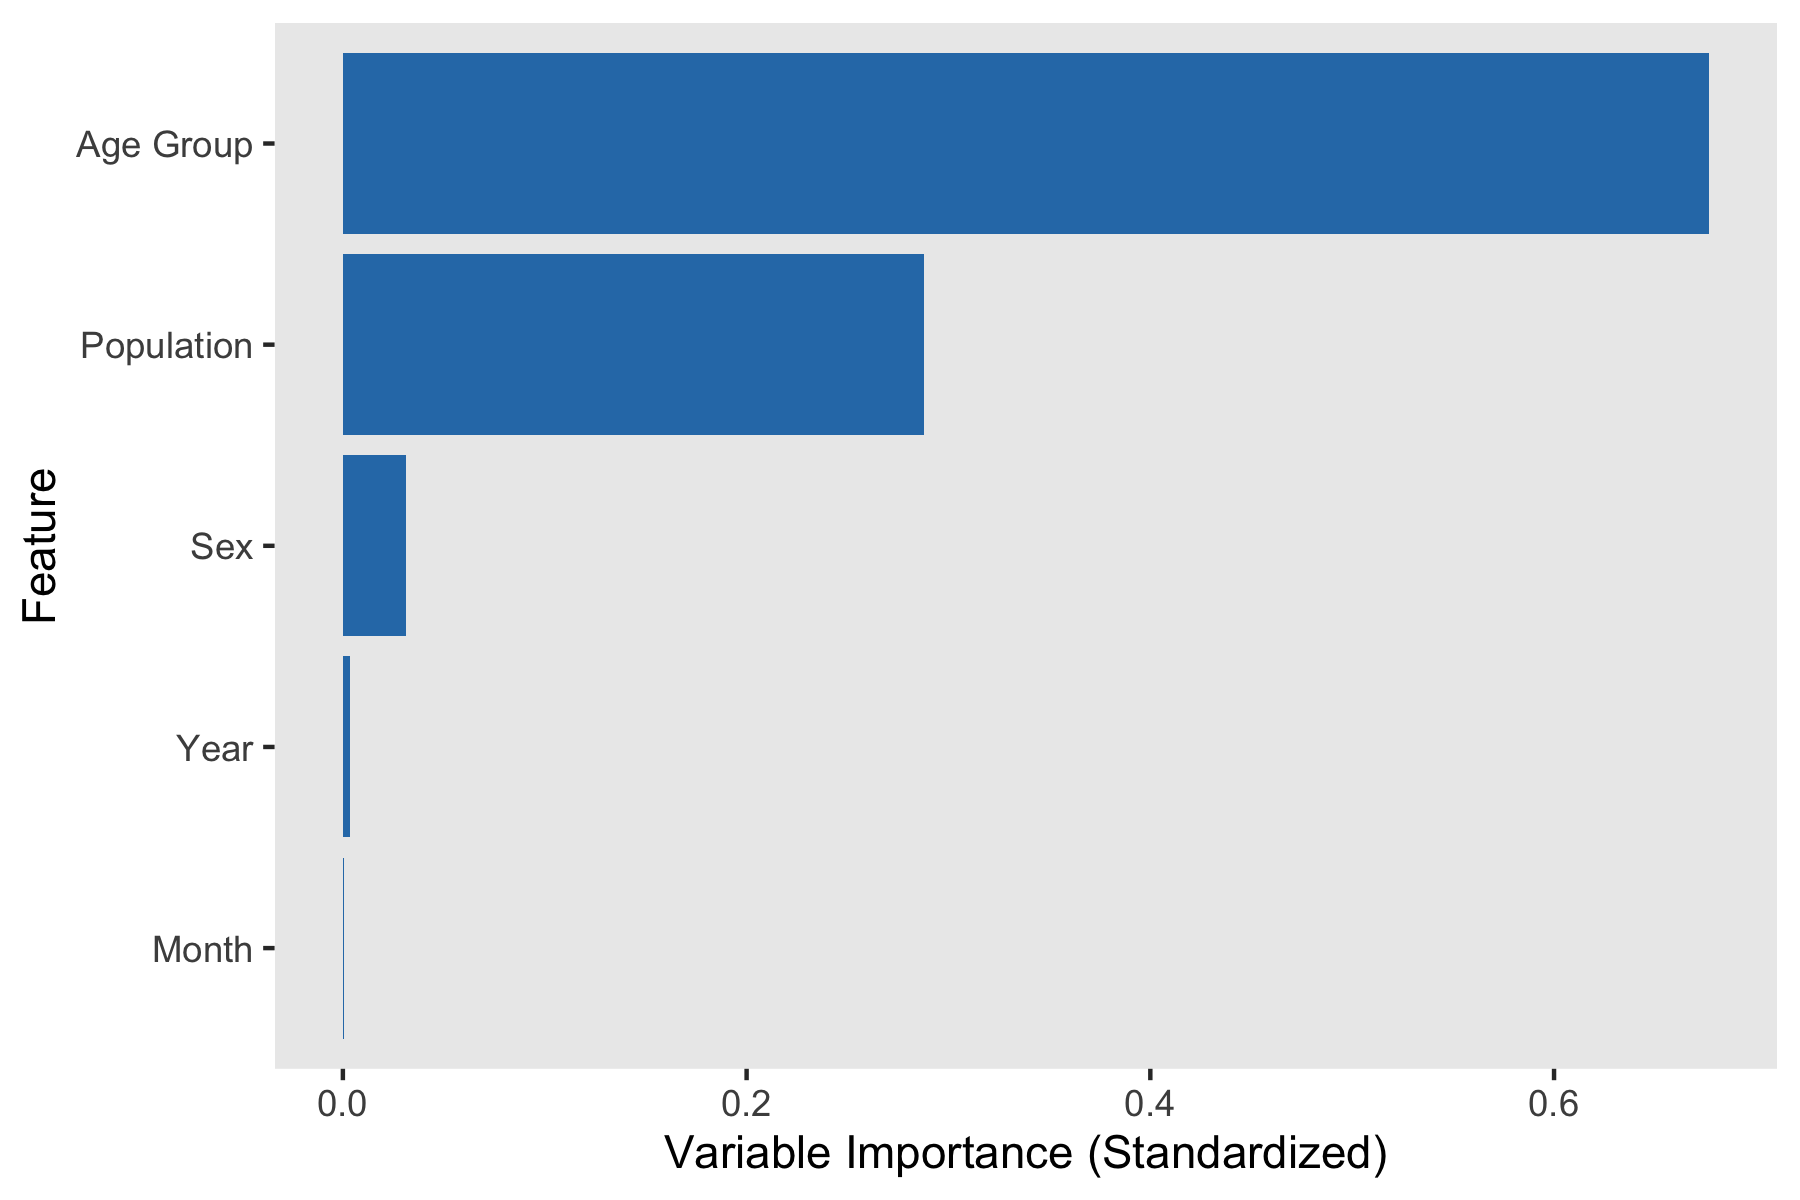
\includegraphics[width = \textwidth]{../figures/vi_rf.png}
        \caption{Random Forest}
         \label{fig:vi_rf}
    \end{subfigure}\hspace{0.02\textwidth}%
    \begin{subfigure}[t]{0.5\textwidth}
        \centering
        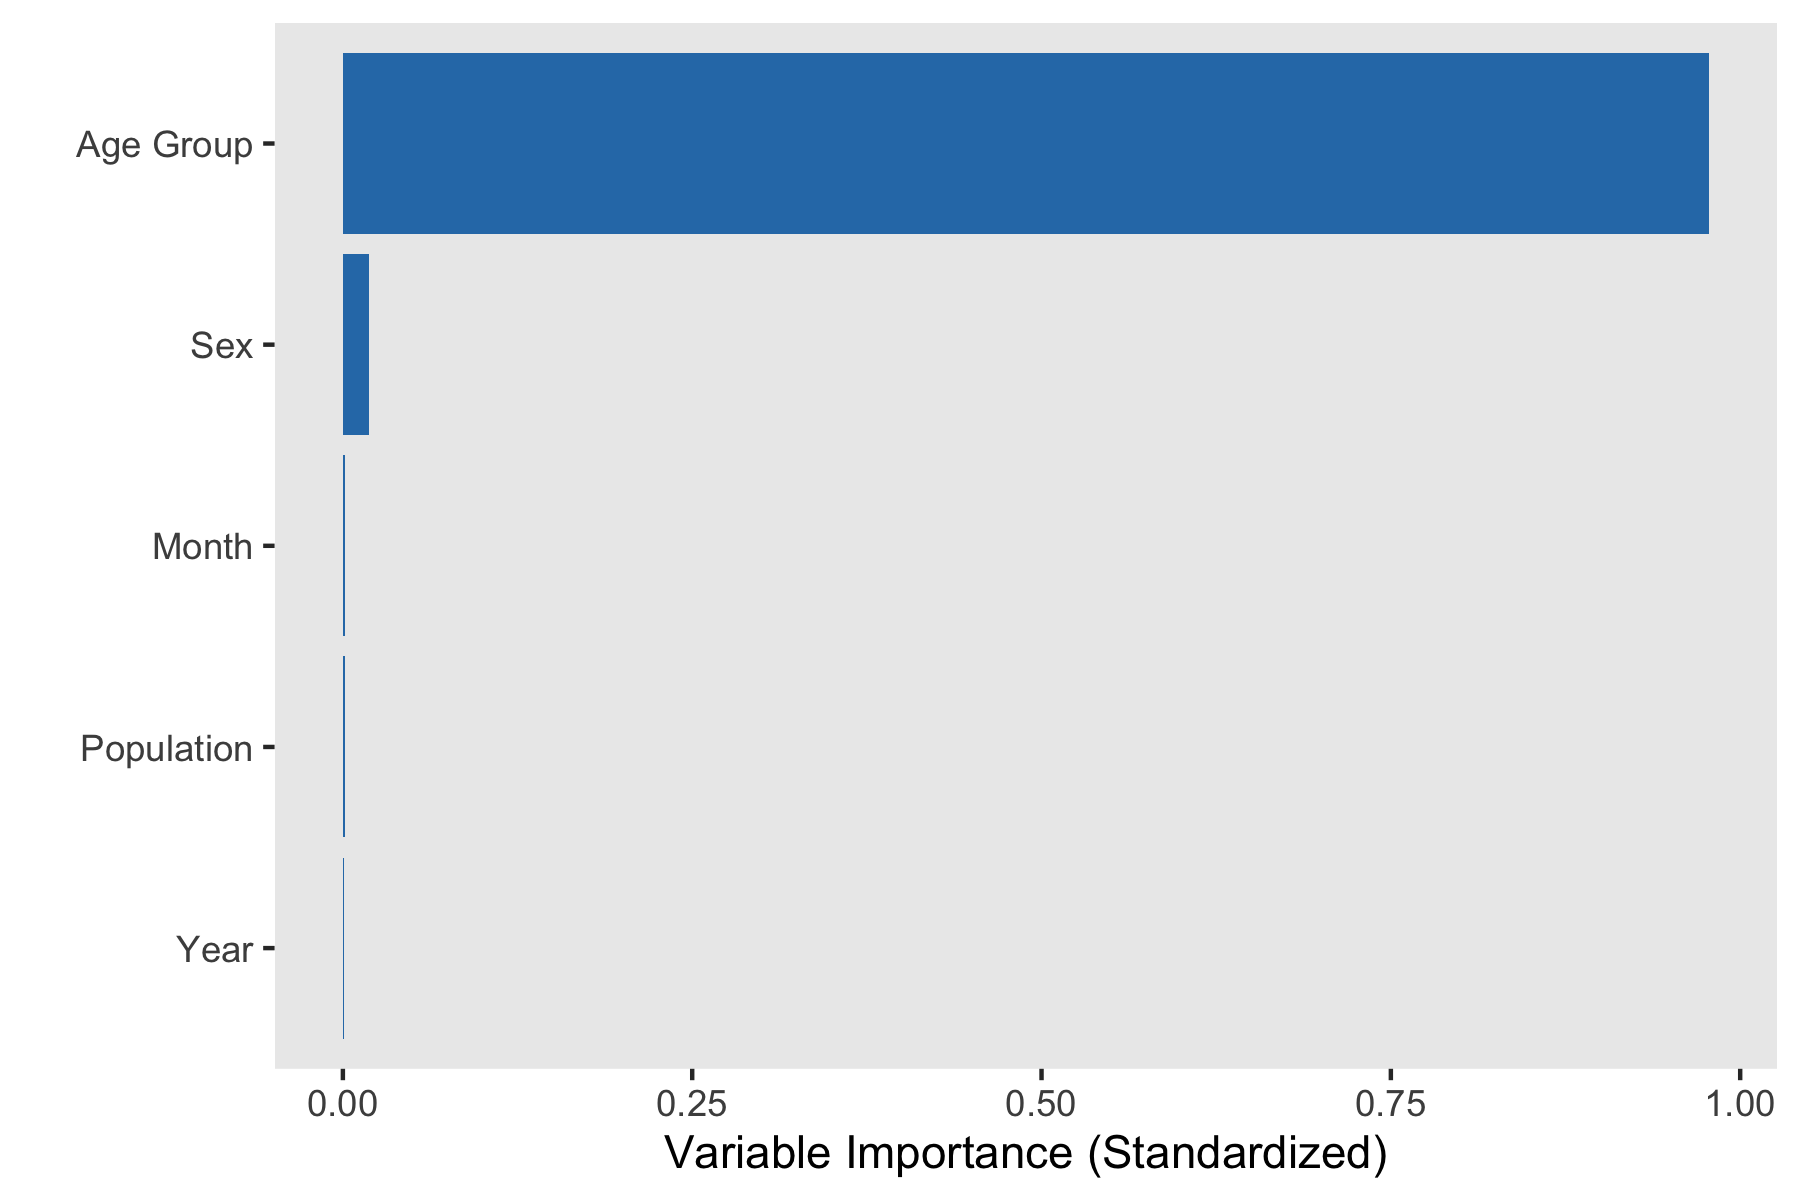
\includegraphics[width = \textwidth]{../figures/vi_gb.png}
         \caption{Gradient Boosting}
         \label{fig:vi_gb}
    \end{subfigure}
    }
     \caption{Relative variable importance for random forest and gradient boosted models.}
\end{figure}


\subsection{Prediction accuracy for demographic groups}

In predicting mortality, a researcher or policy maker would likely want predictions to be accurate for all demographic groups, not just on average, so we are interested in evaluating whether our models are better at predicting mortality for certain groups and not for others. To do this, we calculated a standardized error between the predicted and actual values of mortality on the held-out test set as the absolute value of the difference between the predicted and actual mortality divided by the actual mortality.\footnote{While this wasn't discussed in Stats 600 nor Stats 601, it seemed like an intuitive error to calculate that wouldn't be impacted by the size of the actual mortality rate, and it appears that it is a common error used to measure the accuracy of forecasting models, called the Mean Absolute Percentage Error (MAPE) \cite{mape}.} We then calculate the mean of these standardized errors for each age group and gender combination, across all years and months in the test set.

\begin{figure}[ht]
    \centering
    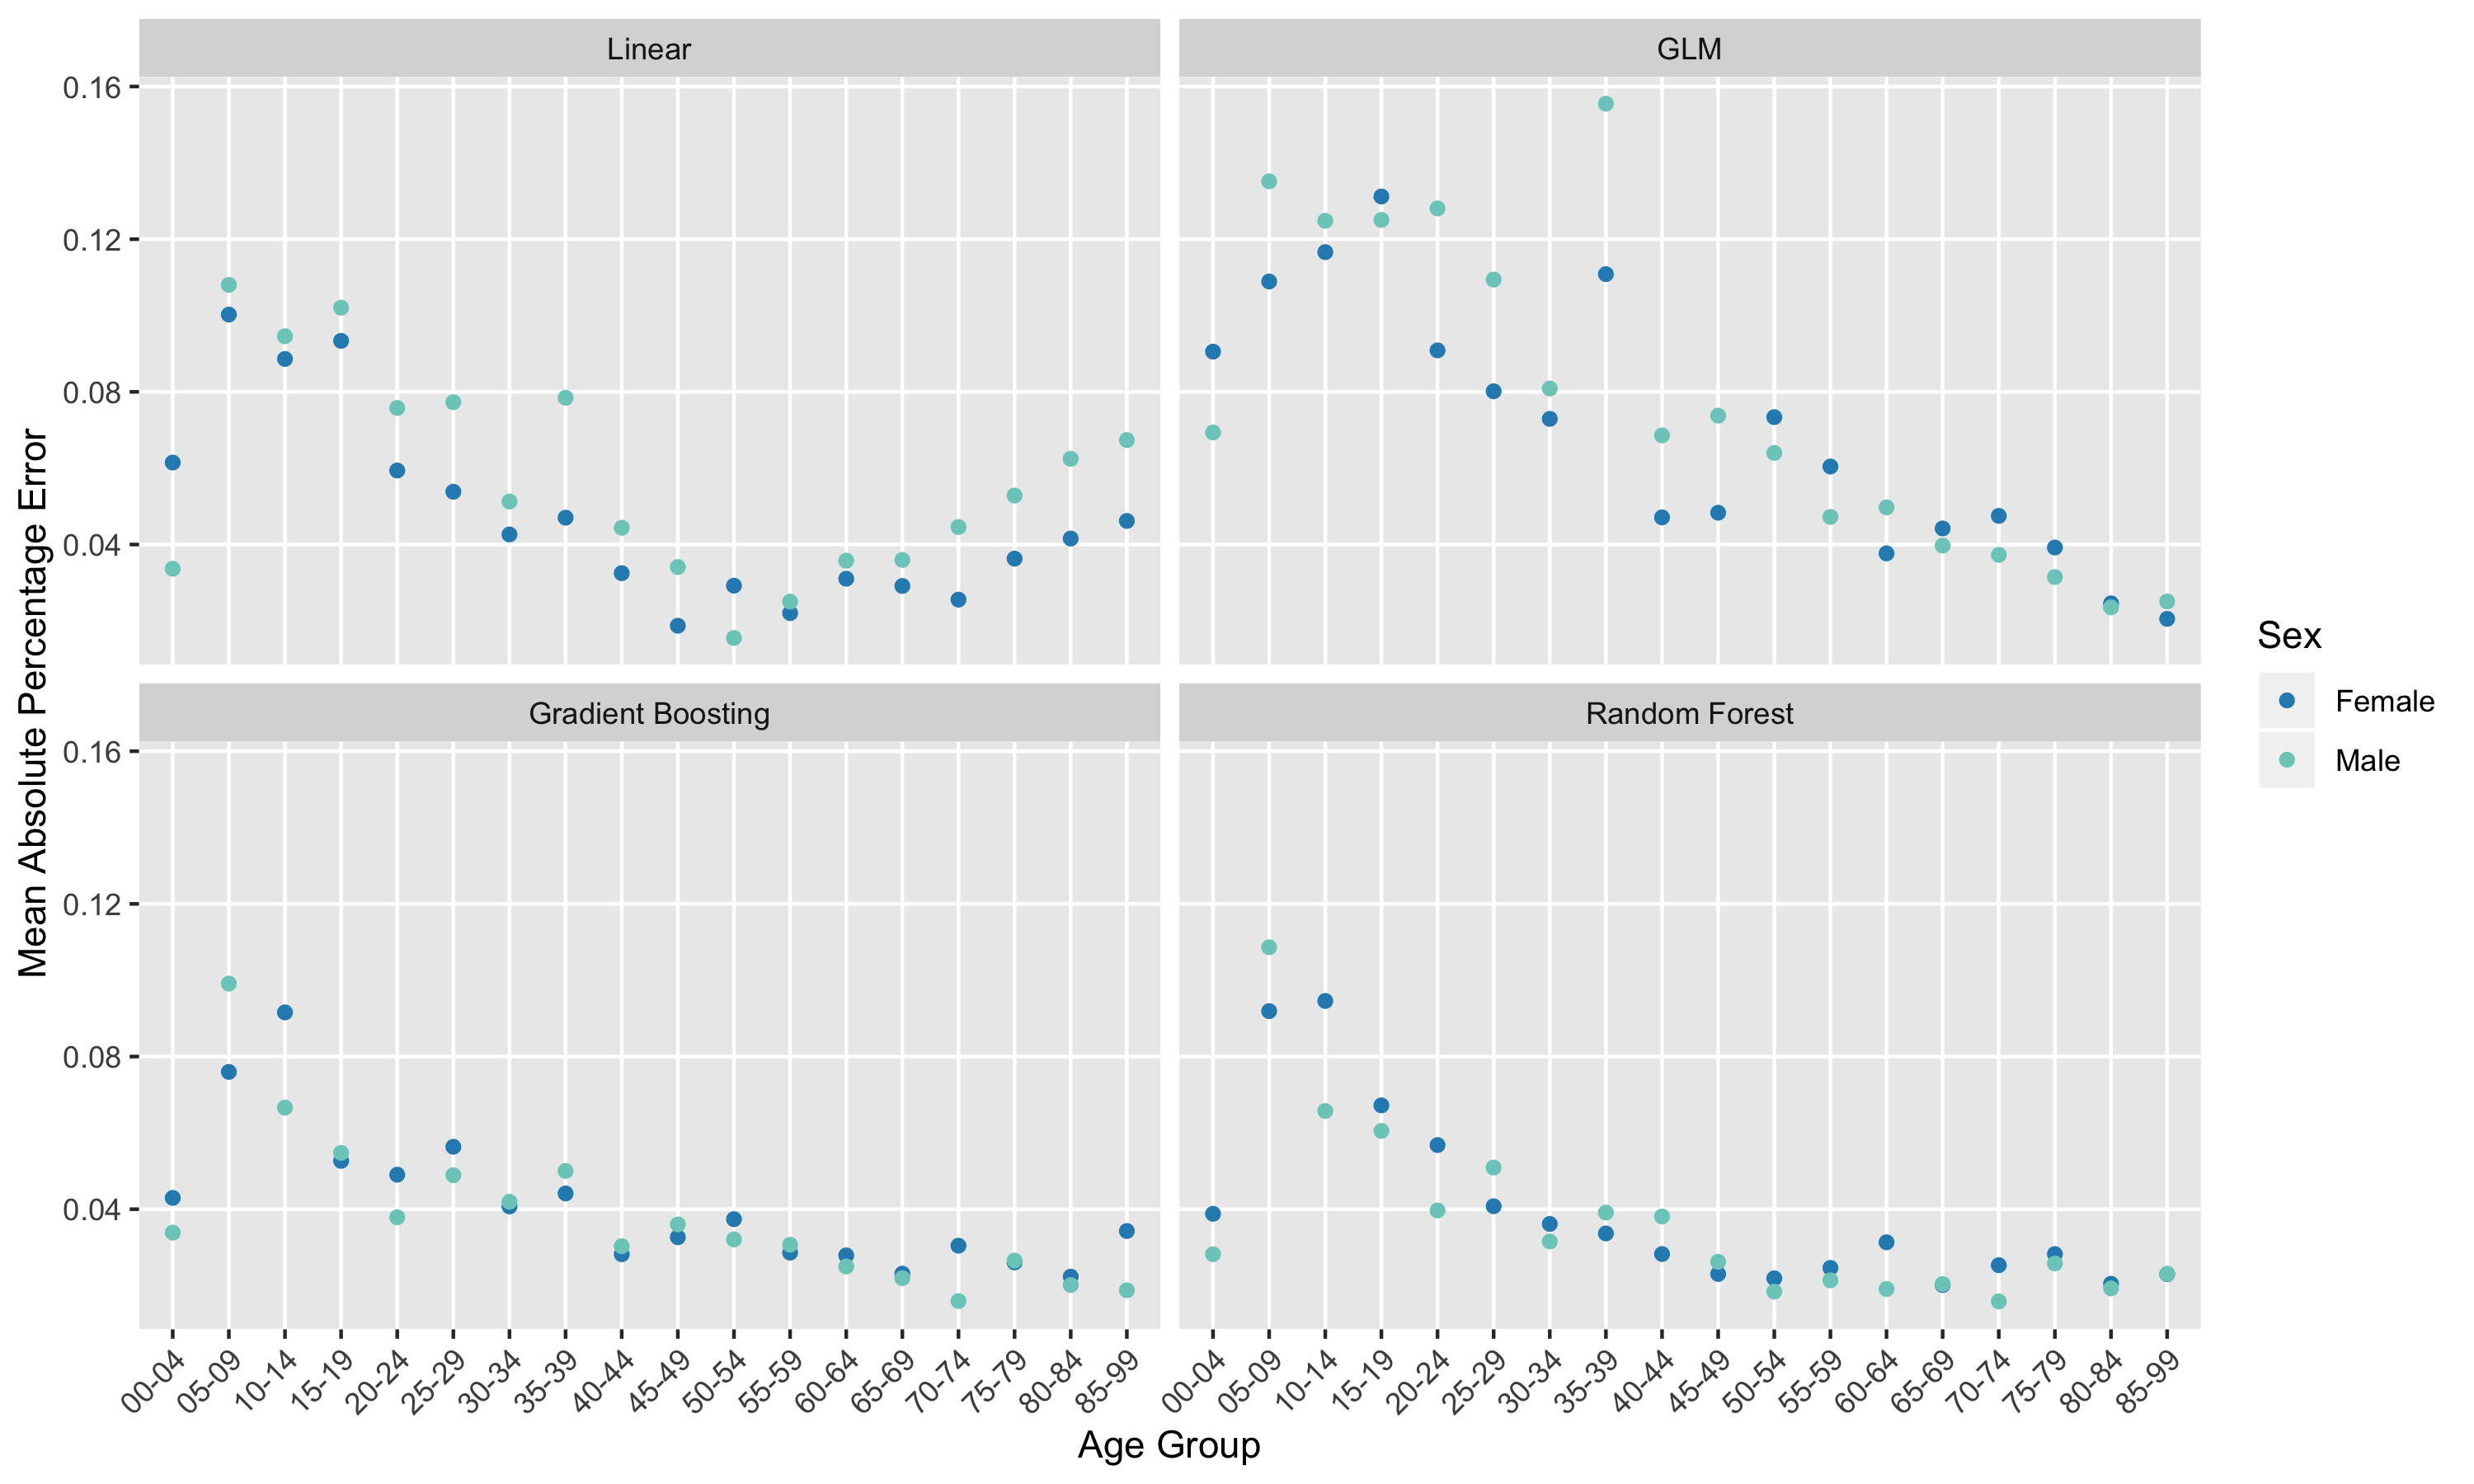
\includegraphics[width = \textwidth]{../figures/err_groups.png}
    \caption{Test mean absolute percentage error by age group and sex for prediction models.}
    \label{fig:mod_err_group}
\end{figure}

\textbf{Figure \ref{fig:mod_err_group}} shows that the four models we use for prediction tend to have higher prediction errors for age groups between 5 and 29 years old. The linear model also has a harder time predicting mortality for older age groups. The relative errors tend to be similar for males and females within the same age group and there is only a noticeable pattern in the prediction error between sexes for the linear model, which tends to have a higher prediction error for males within each age group.  These findings indicate interesting areas for further research, to determine if there are ways to improve the prediction for younger age groups as well as explain the varying behavior of these different models.

\section{Discussion and limitations}

One limitation to this analysis is that we chose to exclude the interaction term between year and month in favor of a simpler model (motivated by BIC). However, an F-test with a significant p-value indicated that the interaction explained some variation in mortality. Therefore, our interpretation for the effect of month on mortality does not consider how the monthly affect varied for different years, and our modeling procedure should not be interpreted to mean that the seasonal effect of month did not vary over time.

Additionally, our analysis has some limitations due to challenges of modeling a highly skewed outcome. First, we did not explore whether the linear model with a log transformation or the GLM with a log link was more appropriate to use given the data, which we would do with more time. Second, the standard measure for evaluating prediction accuracy, MSE, is potentially misleading in this case since the squared error values for observations with high mortality would inherently be larger than squared errors for observations with very low mortality. In addition, because of this, we expected the models that relied on a squared error loss would predict mortality for groups that have higher mortality better than for groups that have lower mortality. We did find that the models tended to have better accuracy for older age groups and lower accuracy for younger age groups.  However, all of this may not matter if one is only interested in minimizing the prediction error of the models in terms of the actual number of people per 100,000 that the model is off by overall. Considering that the average number of deaths per 100,000 people is very small for the age group of 5-9 years (around 1 person), a percentage error of 10\% only means that we could be estimating between .9 and 1.1 people per 100,000, which isn't practically different. We think this data raised interesting questions regarding how to evaluate predictions with highly skewed data and how to improve the models so that the prediction accuracy is similar for groups, regardless of the average magnitude of the response for that group.

Despite the limitations described, through our analysis, we were able to describe and visualize trends in mortality over time and for different demographic groups and how these trends varied by inclusion in certain demographic groups. We also were able to predict monthly mortality using the limited factors available with relatively small overall error. Understanding  trends in mortality is relevant for evaluating health in the U.S. and better targeting groups that appear to have higher risk for dying. For example, one of the striking effects that we found was that the mortality rate for 20 to 24 year old men was predicted to be almost three times that of women of the same age, holding all else constant. This finding suggests further investigation into the factors that cause death for young men. In general, the natural extension of the findings in this report is investigating potential mediating factors that can explain the trends in mortality for different demographic groups.



\bibliography{ref}

\end{document}
